\section{Feasibility experiments}

\subsection{The in-vehicle network}
\todo{Describe that several CAN, LIN \& Ethernet networks exist}
\todo{Describe the three main ECUs (programmable end nodes)}
\todo{Describe the miscellaneous nodes (parametrizable end nodes)}

\subsection{Network traffic}
\todo{Describe that programmable end node traffic is periodic and is defined in data dictionaries and the producer/consumer relationships can be generated easily.}
\begin{table}[htb]
    \centering
    \resizebox{\textwidth}{!}{%
    \begin{tabular}{@{}llllll@{}}
    \toprule
    signal name  & source physical  & source logical           & destination physical   & destination logical         & data type        \\ \midrule
    active\_gear & scu\_primary     & Vehicle Power Controller & scu\_primary           & Braking System Manager      & int16\_t         \\
    power\_mode  & central\_gateway & VPC Gateway              & scu\_primary           & Vehicle Power Controller    & i\_psm\_state\_t \\
    power\_mode  & central\_gateway & VPC Gateway              & scu\_primary           & Energy Storage Controller   & i\_psm\_state\_t \\
    active\_gear & scu\_primary     & Vehicle Power Controller & scu\_primary           & Gear Selector Manager       & int16\_t         \\
    active\_gear & scu\_primary     & Vehicle Power Controller & scu\_primary           & Safety Supervisor Core      & int16\_t         \\
    power\_mode  & central\_gateway & VPC Gateway              & scu\_primary           & Safety Supervisor Core      & i\_psm\_state\_t \\
    active\_gear & scu\_primary     & Vehicle Power Controller & central\_gateway       & Authentication Manager      & int16\_t         \\
    active\_gear & scu\_primary     & Vehicle Power Controller & central\_gateway       & Media ECU Interface Manager & int16\_t         \\
    active\_gear & scu\_primary     & Vehicle Power Controller & central\_gateway       & Lighting Manager            & int16\_t         \\
    active\_gear & scu\_primary     & Vehicle Power Controller & vehicle\_control\_unit & Driver Controls Manager     & int16\_t         \\
    power\_mode  & central\_gateway & VPC Gateway              & vehicle\_control\_unit & Solar Controller            & i\_psm\_state\_t \\
    power\_mode  & central\_gateway & VPC Gateway              & vehicle\_control\_unit & VPC vcu                     & i\_psm\_state\_t \\ \bottomrule
    \end{tabular}%
    }
    \caption{Interface overview for \textit{power\_mode} and \textit{active\_gear} signals}
    \label{tab:interface_overview}
    \end{table}

\begin{figure}[htb]
    \centering
    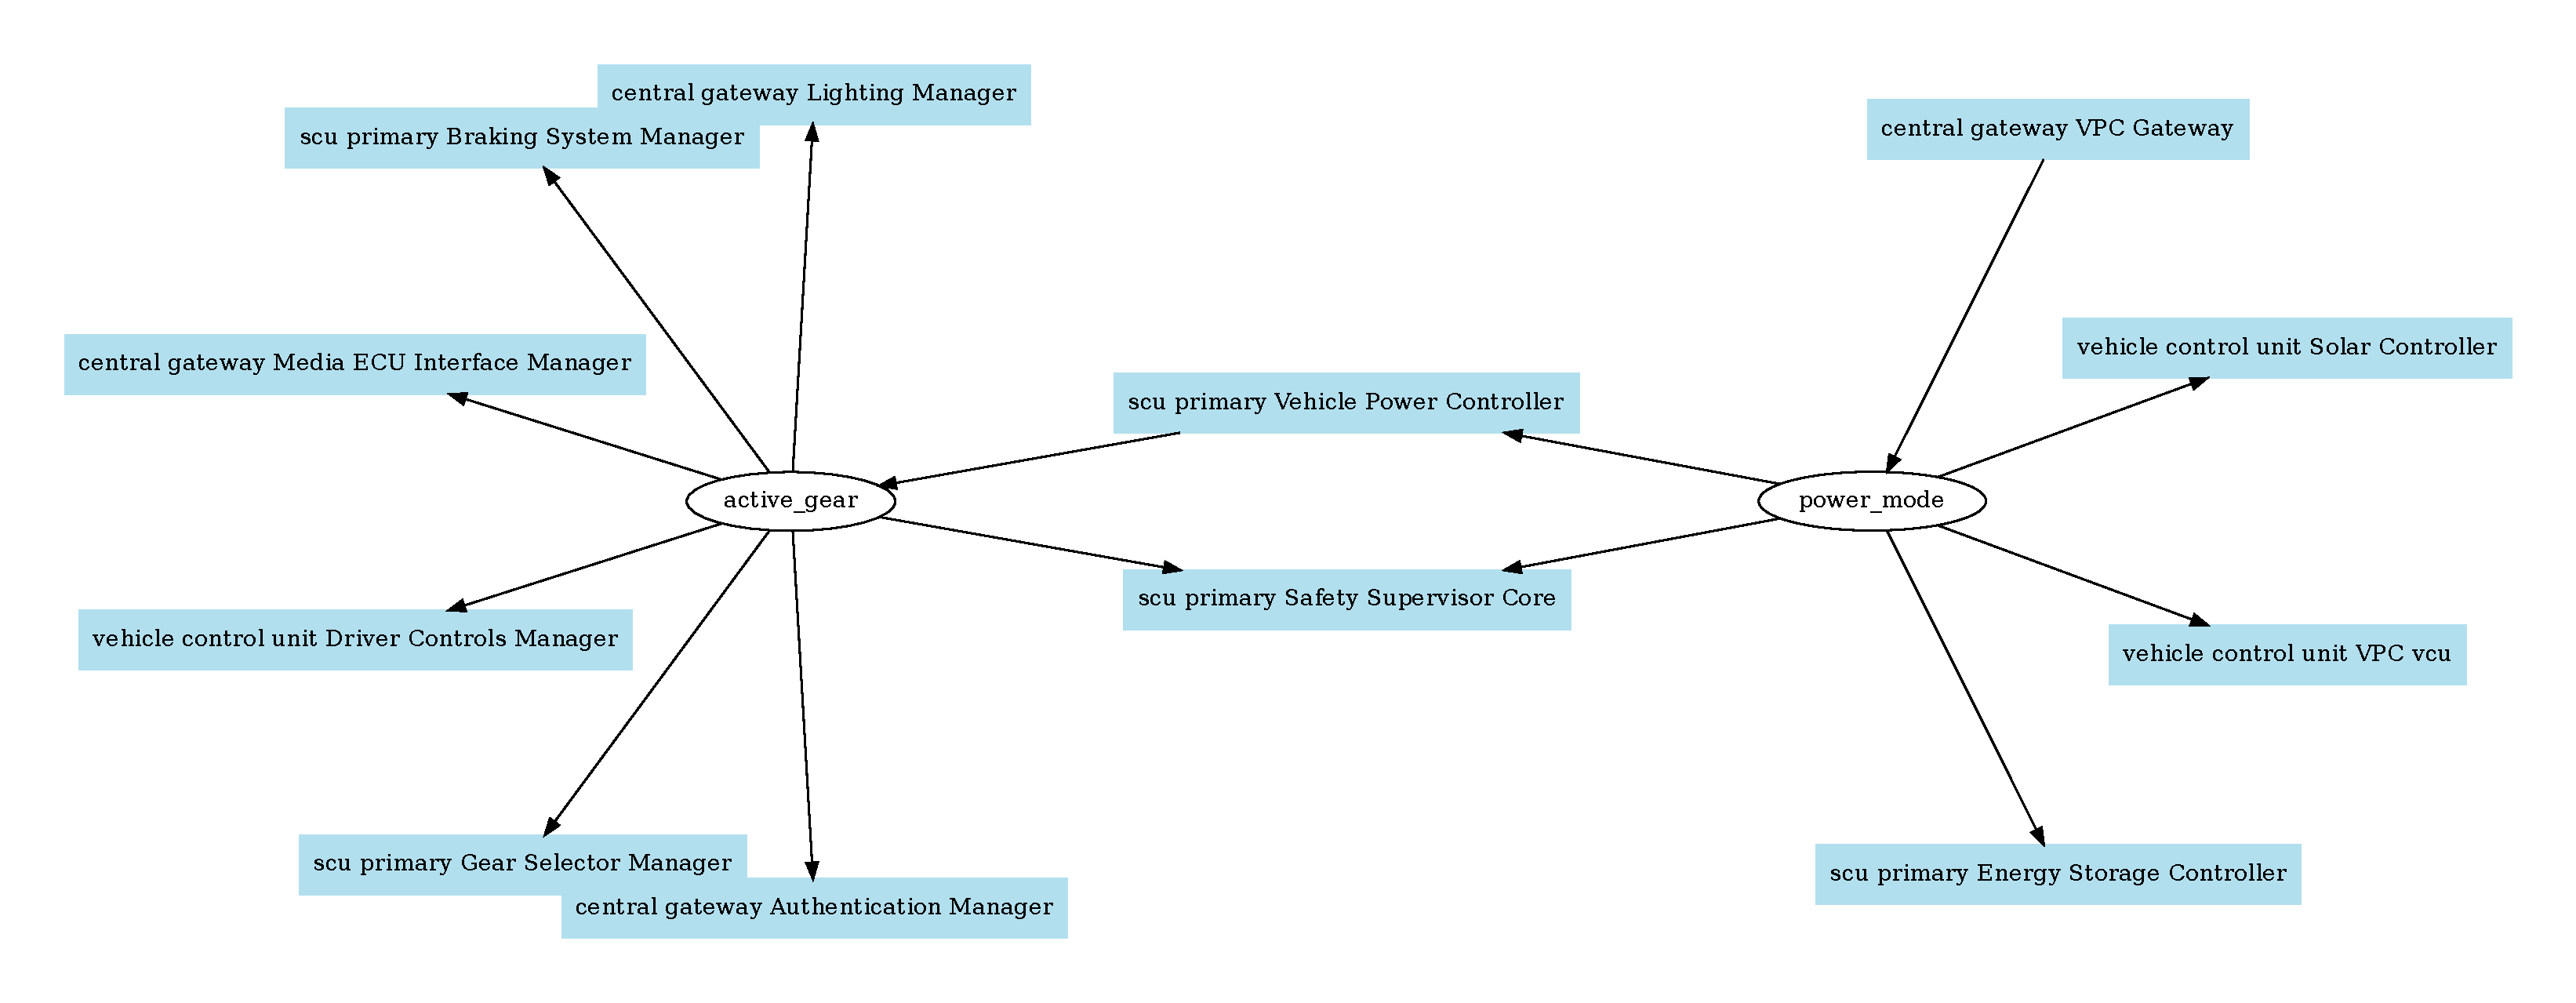
\includegraphics[width=\textwidth]{images/interface_overview.pdf}
    \caption{Interface overview for two signals in graphical form}
    \label{fig:interface_overview}
\end{figure}
\todo{Describe that parametrizable end node traffic is defined in DBC and LDF files, but exact rate is harder to find}
\todo{Describe logging, DTC and update traffic}

\subsection{Discrete Event Simulation in Omnet++}
\begin{figure}[htb]
    \centering
    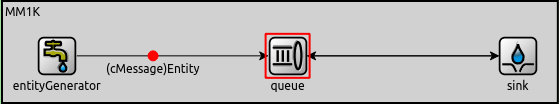
\includegraphics[width=\textwidth]{images/MM1K_sim.png}
    \caption{Visual view of an MM1K queue model in Omnet++}
    \label{fig:mm1k_sim}
\end{figure}
\begin{figure}[htb]
    \centering
    \includegraphics[width=\textwidth]{images/MM1k_analysis.png}
    \caption{Comparison of MM1K queue occupancy between simulation and theoretical analysis}
    \label{fig:MM1K_analysis}
\end{figure}
\todo{Show modelling an MM1K queue}
\todo{Show logical view modelling}
\begin{figure}[htb]
    \centering
    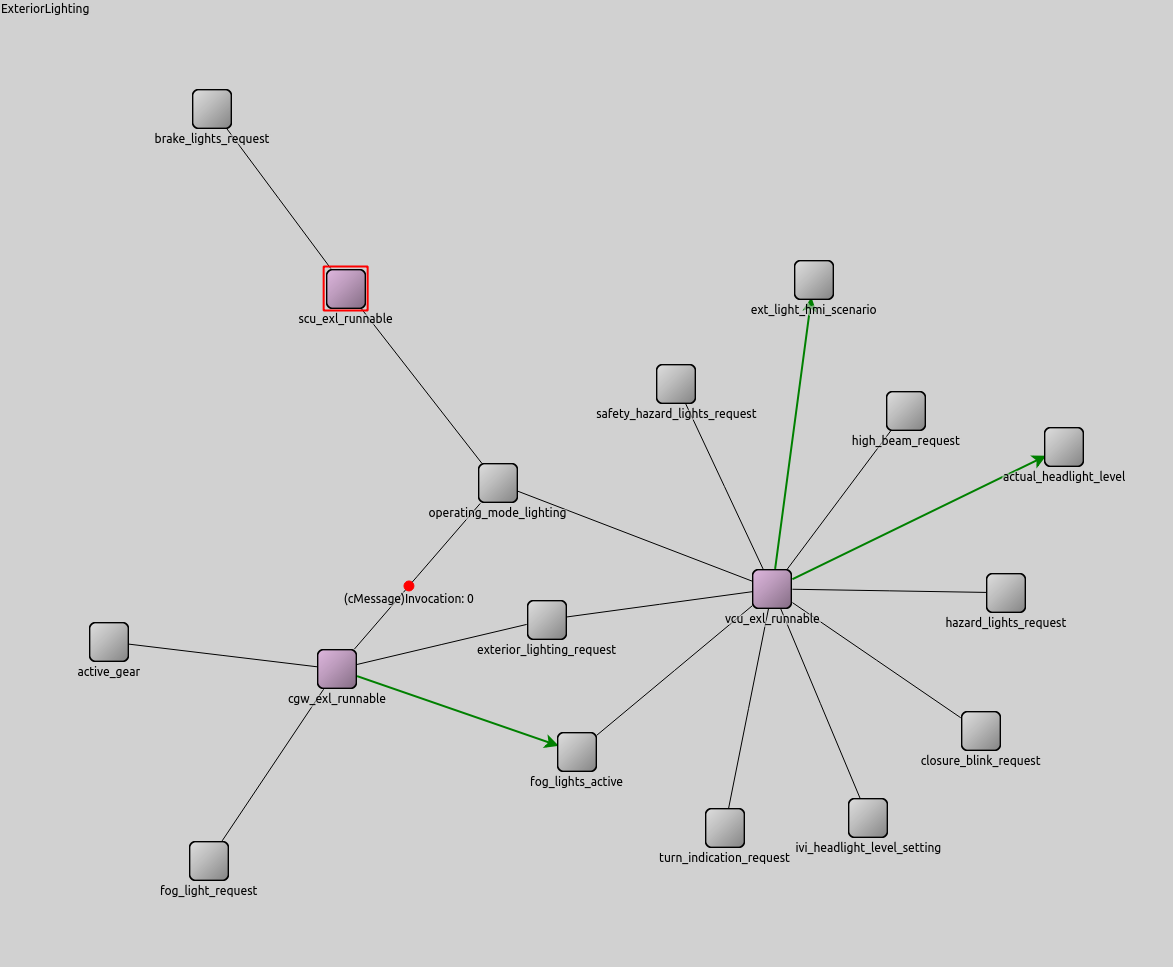
\includegraphics[width=\textwidth]{images/logical_sim.png}
    \caption{Modeling signal transmission of the logical architecture in Omnet++}
    \label{fig:logical_sim}
\end{figure}
\newpage